\begin{center}
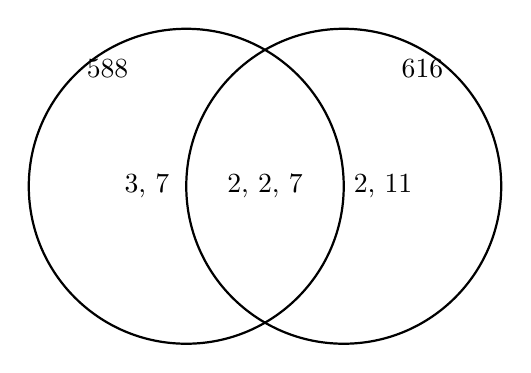
\begin{tikzpicture}
    \begin{scope}
        \tikzset{venn circle/.style={draw, thick, circle, minimum width=4cm}}
        % Draw the sets A and B
        \node [venn circle] (A) at (0,0) {};
        \node [venn circle] (B) at (2,0) {};

        % Label the sets A and B
        \node at (-1, 1.5) {588};
        \node at (3, 1.5) {616};

        % Label each region
        \node at (-0.5, 0) {3, 7}; % Only A
        \node at (2.5, 0) {2, 11}; % Only B
        \node at (1, 0) {2, 2, 7}; % A ∩ B
    \end{scope}
\end{tikzpicture}
\end{center}
